% !TEX root = DesignDocument.tex


\chapter{Overview and concept of operations}

This chapter contains a  general overview of the DanceSoft project. [MB]

\section{Team Members and Team Name}

The DanceSoft Team consist of:
\begin{enumerate}
\item Marcus Berger
\item Dicheng Wu
\end{enumerate}


\section{Client}
The stakeholder and sponsoring customer for this project is Dr. Jeff McGough a computer science professor at the South Dakota School of Mines and Technology and the vice president of the Academy of Dance Arts in Rapid City, South Dakota.
Well not the sponsor of the project Dr. McGough's wife, Julie McFarland is also a key part of the customer base and a stakeholder as the owner and artistic director of the Academy of Dance Arts in Rapid City, South Dakota. The clients main goal is to eventually use the software after some iterations to manage the day to day activities of the Academy, and as the number of iterations of the project increase add student interfaces and refines the project to a point of business viability and security. 



\section{Project}
This first iteration of the project is a proof of concept for the DanceSoft project for purposed use at the Rapid City Academy of Dance Arts. The project after this iteration is meant to be a minimum viable product to give the client as proof of project viability. After this project it will be up to the client, Jeff McGough, to decide whether to keep the project, look elsewhere, or hand over the project to a following senior design team.

As stated above the project is meant to be a minimum viable project, or proof of concept. The system general purpose is running the day to day administrative duties of the Academy of Dance Arts. These duties can range from, but are not necessarily limited to: enter student and class information, payments and billing, or managing employees information. 

\subsection{Purpose of the System}
The purpose of this system is to provide a system for the Academy of Dance Arts to manage their day to day operations, their employees, and their students. These day to day operations range from assigning teachers to classes, looking up information, printing roles sheets for classes, etc.  Also the system must accomplish these task using a user friendly interface, that is as intuitive as possible. The project looks to accomplish this purpose through a local graphical interface and a back end mySQL database for the storage of the data.


\section{Business Need}
The customer needs the team to develop a software solution which can run the dance academy in an effective manner. The product also needs to handle changing classes from year to year without needing to be updated. This means that the software needs to sync with various information, and handle new information such as class rosters, prices, clothing requirements for classes, changes in the employment roster, and many other changes that can occur in the running of the dance school.\\
This project as a whole needs to be an improvement on the current system in use by the customer and provide an easy and efficient way to run the clients business. This project will accomplish the data manipulation task through the back-end MySQL database, and the ease of use will be handled with a simple PyQt interface.
The academy also need the system to work will the employees of the academy which can be devided into admin and teacher categories within the system. The team accomplishes this through a log in system to different landing pages which contain the various functionality completed in this first iteration of the project, as laid out in the user stories listed in this document.
   

\section{Deliverables} 
Listed below are the deliverable major system components for this project. [MB]

\subsection{Major System Component: Database}
The first major component of the system is the MySQL relational database. The database contains the Academy's data and is the core of the back-end side of the software. This database will be the conduit for most of the systems interactions with the data. The database will live within a local computer provided by the user for this first iteration of the software.  

\subsection{Major System Component: User Interface}
The second major component of the system is the front-end user interface for admins and teachers. This will be the only part of the system most users ever see, and will provide an effective means to complete the desired user task. This is accomplished through the use of pages created in PyQt with interfaces to give users effective ways to interact with the database and the necessary data for the requested operations and functions.

\section{Systems Goals}
The system needs to provide a solution which can run the dance studio data and some day to day activities in an effective and secure manner. This includes allowing teachers to print role sheets, look at schedules, and manage their information. Students need to have the ability to see information pertinent to them such as registration and class requirements. Owners and admins need to be able to use the system to manage their employees, the academy's students and it classes, and other administrative duties such as billing. Lastly this system as a whole also needs to be an improvement on the current system in use by the customer and provide an easier and more efficient way to run the clients business.

Overall the system goal is to provide a environment where academy owners, teachers, and students can effectively manage their personal needs and requirements for academy participation and continued operations.

\section{System Overview and Diagram}
\textmd{Users will access this application through a local GUI or a web application depending on their position within the system. The GUI application after client approval or more iterations should reach a final goal of being deployed on the local machines within the Rapid City Academy of Dance Arts. 
When a local GUI user connects the user will navigate through the various pages listed above to the desired functionality. Figure \ref{fig:GUI Overview} shows a simplistic view of the GUI Architecture.
There are two major components to this iteration the project, database, and admin/teacher interface.  Each section is described in more functional detail above and in} \bf section 4 Design and Implementation \rm.
The database architecture is a system of mySQL tables connected through the use of various keys. The tables correspond to the necessary information for various functionality within the system. [MB]


\begin{figure}
  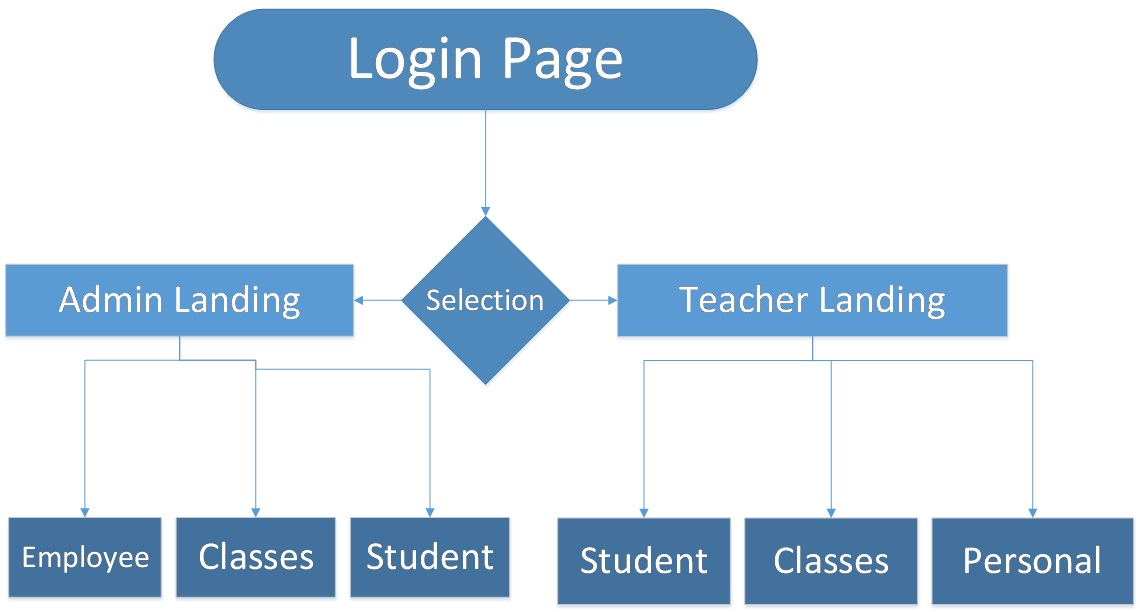
\includegraphics[width=\linewidth]{GUI.jpg}
  \caption{Main GUI Overview}
  \label{fig:GUI Overview}
\end{figure}

\begin{figure}
  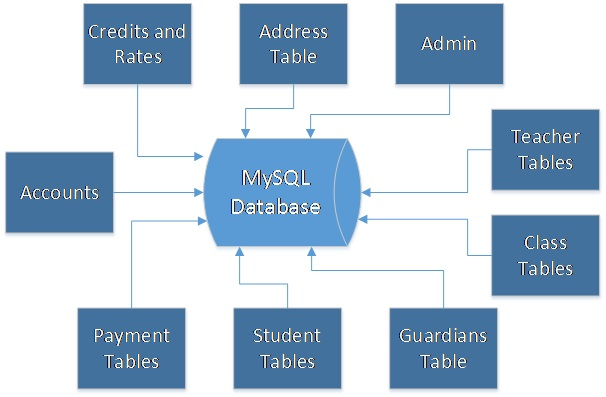
\includegraphics[width=\linewidth]{DatabaseDiagram.jpg}
  \caption{Main Database Overview}
  \label{fig:Database Overview}
\end{figure}


\section{Technologies Overview}
\textmd{The primary Technologies for this projects are as follows:}

\begin{enumerate}
\item Xcode and Visual Studio - Xcode, Microsoft Visual Studio 2015, and Python IDE were the primary development IDEs for this project. Of the three the ones the group used the most were Visual Studio 2015, and the Python IDE so the team could develop the project on the computers provided by the South Dakota School of Mines and Technology. Xcode test were done every so often to confirm the files worked cross-platform.
\item Python - the primary programming language for the project.
\item PyQt and Qt Designer - GUI package and development environment, these tools are publicly available and can be downloaded for free off the internet. 
\item MySQL - MySQL provides the database and relational quires to manage the data and organize it within the system. This software is also free to use and can be downloaded from the MySQL website.
\end{enumerate}




\textmd{These technologies were selected after a first research sprint where research into programming language, GUI, and database options was conducted and the technologies were selected. A brief description of the research can be found in the sprint 1 report or the first prototype sections of this document. [MB]}

